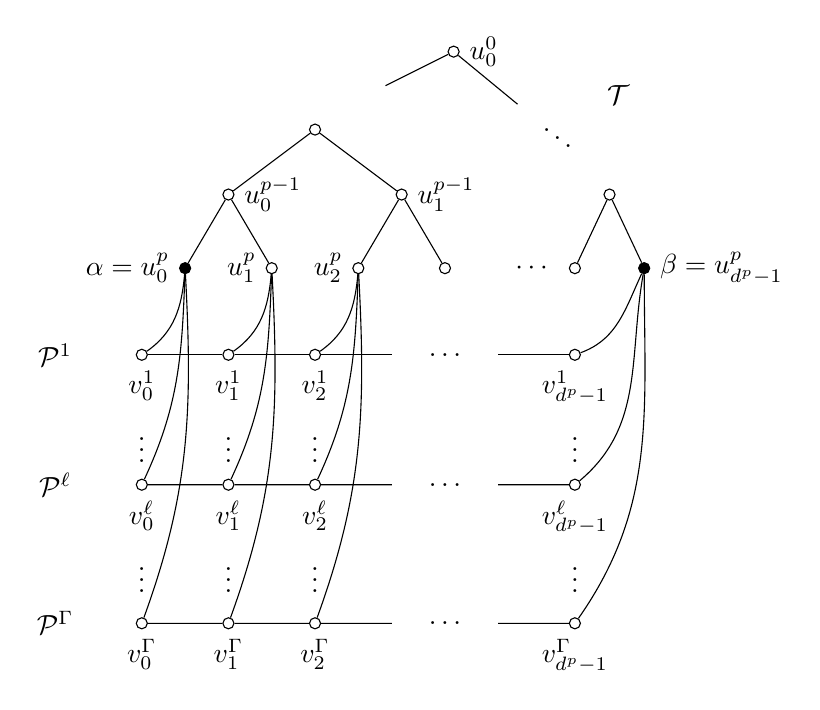
\begin{tikzpicture}[scale=1.1]
    % Define styles for different types of vertices
    \tikzset{
        vertex/.style={circle, draw, minimum size=4pt, inner sep=1pt, fill=white},
        filled/.style={circle, draw, fill=black, minimum size=4pt, inner sep=1pt},
    }
    
    
    % Draw vertices on level A with labels
    \node[] at (-1,0) {$\mathcal{P}^1$};
    \node[vertex] (a) at (0,0) [label=below:$v^1_0$] {};
    \node[vertex] (b) at (1,0) [label=below:$v^1_1$] {};
    \node[vertex] (c) at (2,0) [label=below:$v^1_2$] {};
    \node[] (ca) at (3,0) {};
    \node[] at (3.5,0) {$\dots$};
    \node[] (cb) at (4,0) {};
    \node[vertex] (d) at (5,0) [label=below:$v^1_{d^p-1}$] {};

    \node (dda) at (0,-1) {$\vdots$};
    \node (ddb) at (1,-1) {$\vdots$};
    \node (ddc) at (2,-1) {$\vdots$};
    \node (ddd) at (5,-1) {$\vdots$};
    \node (ddda) at (0,-2.5) {$\vdots$};
    \node (dddb) at (1,-2.5) {$\vdots$};
    \node (dddc) at (2,-2.5) {$\vdots$};
    \node (dddd) at (5,-2.5) {$\vdots$};
    
    % Draw vertices on level B with labels
    \node[] at (-1,-1.5) {$\mathcal{P}^\ell$};
    \node[vertex] (e) at (0,-1.5) [label=below:$v^\ell_0$] {};
    \node[vertex] (f) at (1,-1.5) [label=below:$v^\ell_1$] {};
    \node[vertex] (g) at (2,-1.5) [label=below:$v^\ell_2$] {};
    \node[] (ga) at (3,-1.5) {};
    \node[] at (3.5,-1.5) {$\dots$};
    \node[] (gb) at (4,-1.5) {};
    \node[vertex] (h) at (5,-1.5) [label=below:$v^\ell_{d^p-1}$] {};
    
    % Draw vertices on level C with labels
    \node[] at (-1,-3.1) {$\mathcal{P}^\Gamma$};
    \node[vertex] (i) at (0,-3.1) [label=below:$v^\Gamma_0$] {};
    \node[vertex] (j) at (1,-3.1) [label=below:$v^\Gamma_1$] {};
    \node[vertex] (k) at (2,-3.1) [label=below:$v^\Gamma_2$] {};
    \node[] (ka) at (3,-3.1) {};
    \node[] at (3.5,-3.1) {$\dots$};
    \node[] (kb) at (4,-3.1) {};
    \node[vertex] (l) at (5,-3.1) [label=below:$v^\Gamma_{d^p-1}$] {};
    
    % Draw tree structure vertices
    \node at (5.5,3) {$\mathcal{T}$};
    \node[vertex] (o) at (3.6,3.5) [label=right:$u_0^0$] {};
    
    \node (left) at (2.7,3.05) {};
    \node (right) at (4.45,2.8) {};
    
    \node (eleft) at (2.45,3) {$\iddots$};
    \node (eright) at (4.8,2.6) {$\ddots$};
    \node[vertex] (pq) at (2,2.6) {};
    
    \node[vertex] (p) at (1,1.85) [label=right:$u^{p-1}_0$] {};
    \node[vertex] (q) at (3,1.85) [label=right:$u^{p-1}_1$] {};
    \node[vertex] (qq) at (5.4,1.85) {};
    
    \node[filled] (s) at (0.5,1) [label=left:{$\alpha=u^p_0$}] {};
    \node[vertex] (m) at (1.5,1) [label=left:$u^p_1$] {};
    \node[vertex] (n) at (2.5,1) [label=left:$u^p_2$] {};
    \node[vertex] (nn) at (3.5,1) {};
    \node (mid) at (4.5,1) {$\cdots$};
    \node[vertex] (rl) at (5,1) {};
    \node[filled] (r) at (5.8,1) [label=right:{$\beta=u^p_{d^p-1}$}] {};
    
    % Draw path connections
    \draw (a) -- (b) -- (c) -- (ca);
    \draw (e) -- (f) -- (g) -- (ga);
    \draw (i) -- (j) -- (k) -- (ka);
    \draw (cb) -- (d);
    \draw (gb) -- (h);
    \draw (kb) -- (l);
    
    % Draw tree connections
    \draw (o) -- (left);
    \draw (o) -- (right);
    \draw (p) -- (pq);
    \draw (q) -- (pq);
    \draw (p) -- (s);
    \draw (p) -- (m);
    \draw (q) -- (n);
    \draw (q) -- (nn);
    \draw (qq) -- (r);
    \draw (qq) -- (rl);
    
    \draw (s) to [out=265, in=35] (a);
    \draw (s) to [out=268, in=65] (e);
    \draw (s) to [out=273, in=70] (i);
    \draw (m) to [out=265, in=35] (b);
    \draw (m) to [out=268, in=65] (f);
    \draw (m) to [out=273, in=70] (j);
    \draw (n) to [out=265, in=35] (c);
    \draw (n) to [out=268, in=65] (g);
    \draw (n) to [out=273, in=70] (k);
    \draw (r) to [out=245, in=20] (d);
    \draw (r) to [out=260, in=40] (h);
    \draw (r) to [out=270, in=55] (l);
\end{tikzpicture}